\subsection{Model Validation}
\label{subsec:model_validation}

Achieving a good in-sample fit does not necessarily guarantee that our model will also
be able to make out of sample predictions. For example, it could be that the results
are very sensitive to the exact number of vaccinations, the work mobility multiplier
or the number of rapid tests that are performed -- all of which are things that cannot
be exactly known ex-ante.

In this section we compare simulated infections that use all available data with
out of sample predictions that only use data that was available at March 1 2021.

For the out of sample predictions we predict the number of vaccinations between March
and June with a simple linear regression model that was fitted on vaccine data from
February. This prediction model is pessimistic compared to the actual number of
vaccinations. The work mobility multiplier is predicted to be constant at a value of
0.75, which is an approximate average of the second half of February. This turned out
to be optimistic.

The area that is fraught with the most uncertainty is the introduction of rapid test,
because it comprises both supply and demand factors. Moreover, accurately predicting
the number of rapid tests is expected to be important because rapid tests play a large
role for the transmission dynamic.

We therefore make a scenario analysis with different assumptions on the availability
of rapid tests. The number of rapid tests performed in each scenario can be seen in
Figure~\ref{fig:robustness_check_rapid_test_params}. All scenarios are the same
unti March 1 and have the same level of rapid tests when all supply constraints are
resolved. They differ in the date at which the full number of tests is reached. For
students and teachers the full number of rapid tests is reached after the easter
holidays. For rapid tests in the workplace and private rapid tests it is reached between
May 1 and June 10, depending on the scenario.


\begin{figure}[ht] % Robustness Check Rapid Test Fade In Params
  \centering
  \begin{subfigure}[b]{0.3\textwidth}
    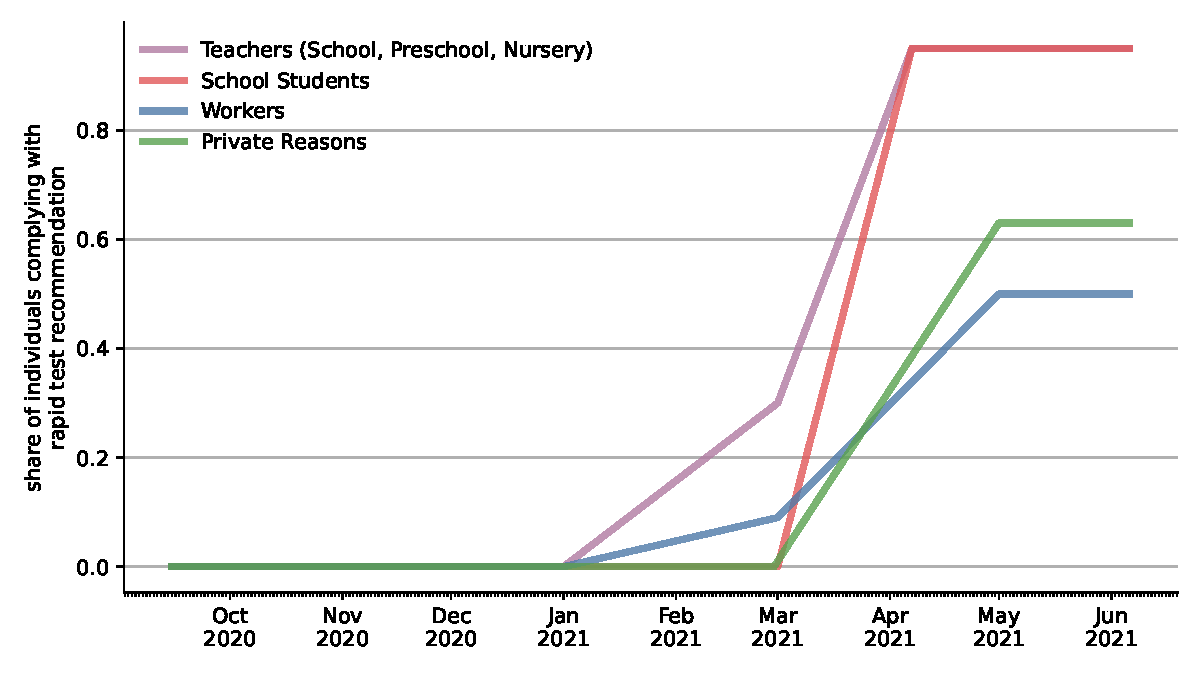
\includegraphics[width=\textwidth]{figures/results/figures/data/testing/rapid_test_demand/robustness_check_params_early_shares}
    \caption{Rapid Test Parameters: Early Scenario}
    \label{fig:robustness_early_params}
  \end{subfigure}
  \hfill
  \begin{subfigure}[b]{0.3\textwidth}
    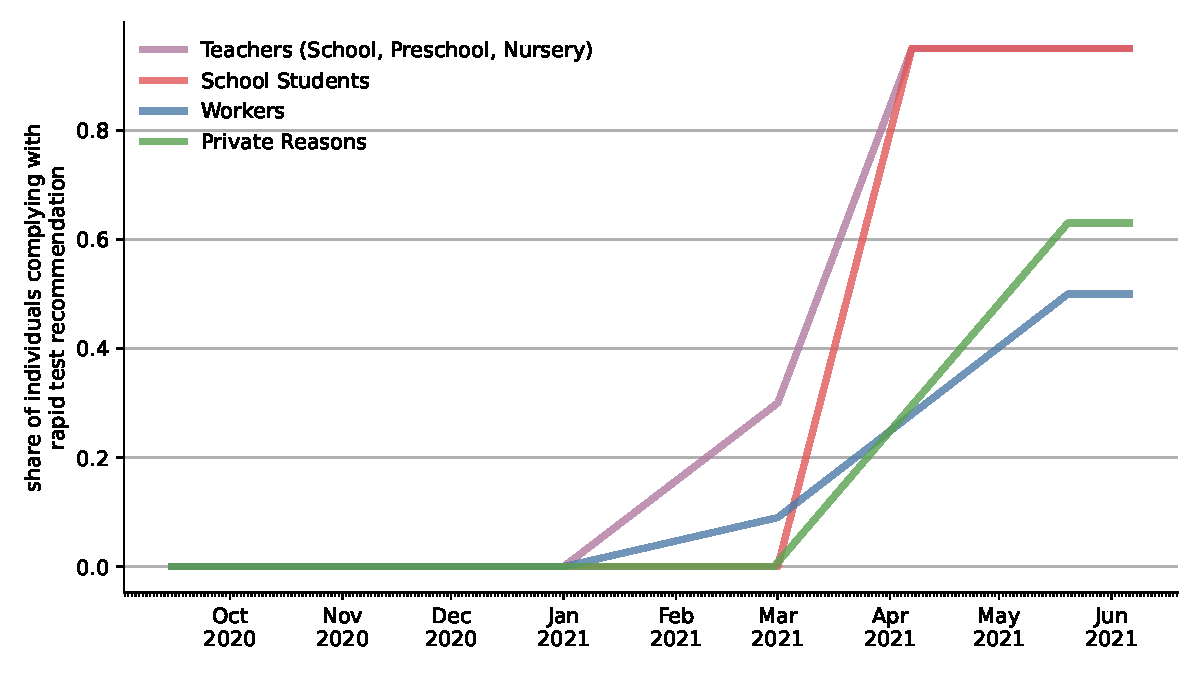
\includegraphics[width=\textwidth]{figures/results/figures/data/testing/rapid_test_demand/robustness_check_params_medium_shares}
    \caption{Rapid Test Parameters: Medium Scenario}
    \label{fig:robustness_medium_params}
  \end{subfigure}
  \hfill
  \begin{subfigure}[b]{0.3\textwidth}
    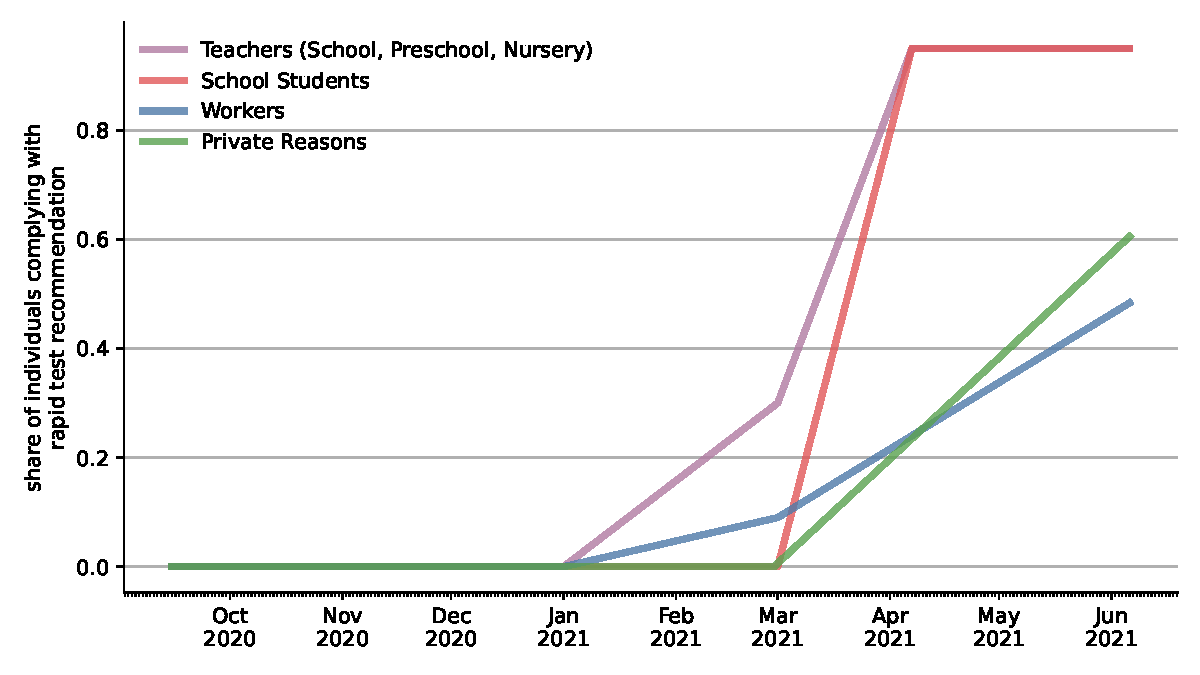
\includegraphics[width=\textwidth]{figures/results/figures/data/testing/rapid_test_demand/robustness_check_params_late_shares}
    \caption{Rapid Test Parameters: Late Scenario}
    \label{fig:robustness_late_params}
  \end{subfigure}

  \caption{Rapid Test Introduction in the Three Scenarios}
  \label{fig:robustness_check_rapid_test_params}

  \floatfoot{\noindent \textit{Note:} Number of rapid tests performed in the different
  prediction scenarios. All scenarios are the same
  unti March 1 and have the same level of rapid tests when all supply constraints are
  resolved. They differ in the date at which the full number of tests is reached. For
  students and teachers the full number of rapid tests is reached after the easter
  holidays. For rapid tests in the workplace and private rapid tests it is reached
  between May 1 and June 10, depending on the scenario.
  }
\end{figure}

Moreover, the out of sample predictions assume that the share of detected cases that
would have obtained without rapid tests is not affected by the easter holidays because
the extent to which this was the case was estimated from case numbers in April.

The results of the out of sample prediction are displayed in
Figure~\ref{fig:robustness_check_detailed}. While all scenarios considerably deviate from
the ex-post scenario, they all reproduce the steep increase of cases until the end
of April, followed by a decline until June. We can therefore conclude that our main
results are not sensitive to measurement errors in the number of rapid tests,
vaccinations or mobility data.


\begin{figure}[ht] % Robustness Check
  \centering
  \begin{subfigure}[b]{.425\textwidth}
    \centering
    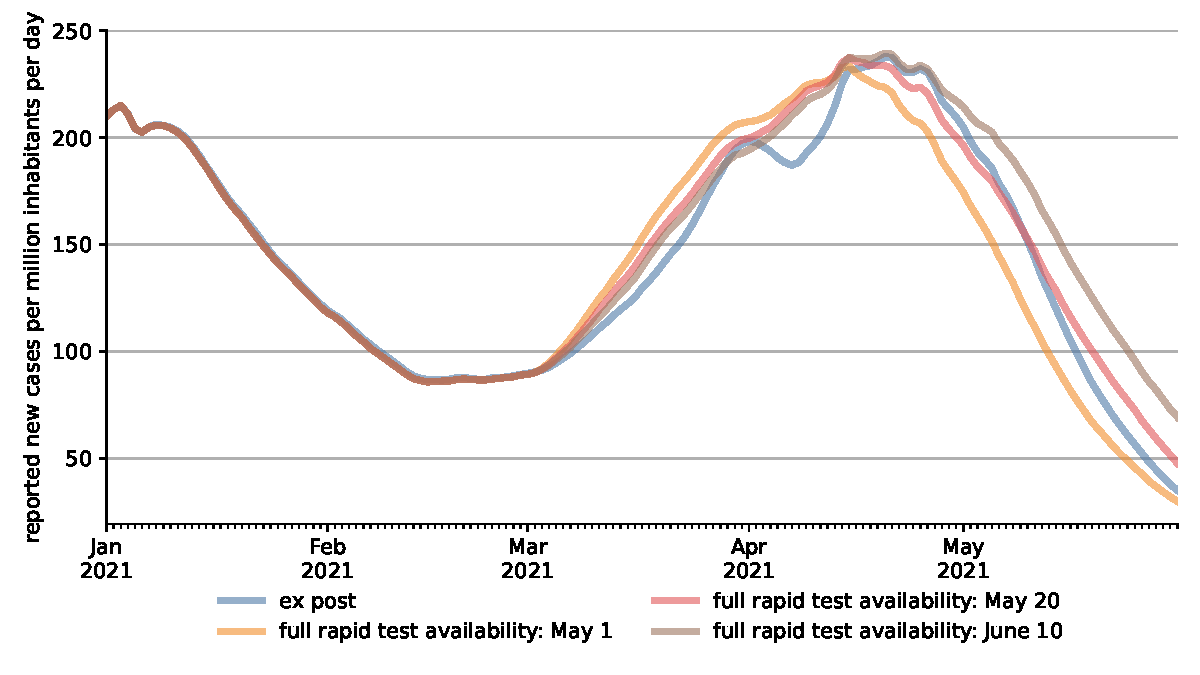
\includegraphics[width=\textwidth]{figures/results/figures/scenario_comparisons/robustness_check/full_new_known_case}
    \caption{Reported Cases}
    \label{fig:robustness_check_new_known_case}
  \end{subfigure}%
  \hfill
  \begin{subfigure}[b]{.425\textwidth}
    \centering
    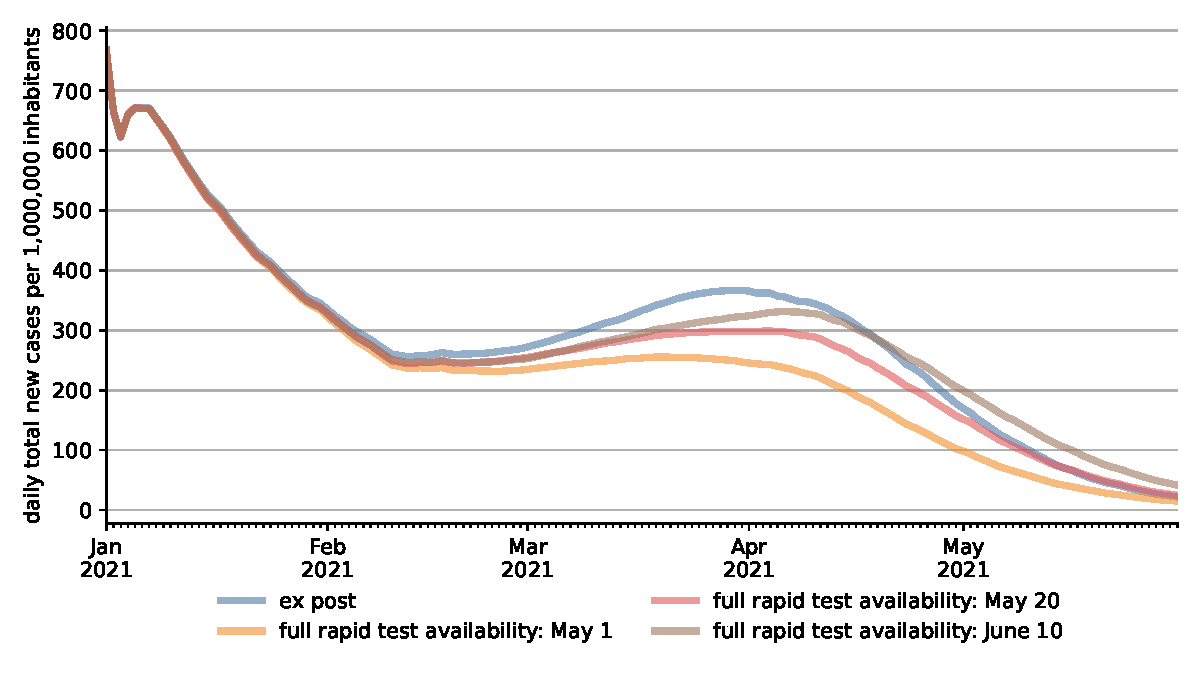
\includegraphics[width=\textwidth]{figures/results/figures/scenario_comparisons/robustness_check/full_newly_infected}
    \caption{Total Cases}
    \label{fig:robustness_check_newly_infected}
  \end{subfigure}
  \caption{Out of Sample Prediction for Reported and Total Cases from March to June
  2021.}
  \label{fig:robustness_check_detailed}
  \floatfoot{\noindent \textit{Note:} The ex-post scenario is an in-sample prediction
  that uses all available information and is very close to actual case numbers. For the
  other scenarios data on vaccinations, work mobility and rapid tests that became
  available after March 1 have been replaced by prediction models that are calibrated
  with data from February. Moreover, they do not model a lower number of detected cases
  over the easter holidays. The different scenarios make different assumptions on the
  date at which full availability of rapid tests is reached. While the out of sample
  predictions differ substantially for the exact case numbers at the beginning of June
  (between 20 and 70 cases per million), they can all reproduce the decline in case
  numbers that is jointly driven by seasonality, large scale rapid tests and
  vaccinations.}
\end{figure}

\FloatBarrier
